\documentclass[conference]{IEEEtran}

\usepackage[T1]{fontenc}
\usepackage{cite}
\usepackage{amsmath}
\usepackage{booktabs}
\usepackage{array}
\usepackage{graphicx}
\usepackage{url}
\usepackage{tikz}
\usepackage{pgfplots}
\usetikzlibrary{arrows.meta,positioning,fit}
\pgfplotsset{compat=1.18}
\definecolor{modelteal}{RGB}{18,108,112}
\definecolor{modelorange}{RGB}{184,93,45}
\definecolor{modelviolet}{RGB}{122,94,160}

\title{A Reproducible Flow-Based Intrusion Detection Study with Uncertainty-Directed Review under Feature Outages}

% Replace the author and affiliation placeholders before submission.
\author{\IEEEauthorblockN{Your Name}
\IEEEauthorblockA{Department or Program\\
University or Institution\\
City, Country\\
email@example.com}}

\begin{document}
\maketitle

\begin{abstract}
Network intrusion classifiers are commonly summarized by a single test-set score, even though operational review capacity is limited and flow measurements may be missing. This paper describes CyberSentinel-ML, a reproducible binary-classification and review prototype built around the official UNSW-NB15 training and testing split. The implementation compares Random Forest, Bagging, and Gradient Boosting pipelines, then evaluates a separate question: when an entire group of flow features is unavailable at inference time, does uncertainty-ranked review identify more classification errors than random review at the same workload, and does that pattern differ by attack category? At a fixed decision threshold of 0.55, Bagging achieved the highest attack F1-score (0.9209), Gradient Boosting the highest accuracy (0.9092), and Random Forest the highest attack recall (0.9819). In the clean-feature triage scenario, a 10\% review budget captured a mean of 3,891.8 errors across five Random Forest seeds, compared with 976.0 errors for same-size random review. The paired seed-level sign test yielded $p=0.0625$; the adjusted value was $q=0.0948$. Thus, the observed lift is practically large on this benchmark split but does not meet a 0.05 significance threshold under the reported correction. Category-level results varied, and rare categories contained too few errors for stable conclusions. The contribution is an auditable evaluation workflow and a cautious empirical analysis, rather than a new classifier or a claim of generalization to live networks.
\end{abstract}

\begin{IEEEkeywords}
network intrusion detection, UNSW-NB15, feature outage, uncertainty sampling, human review, ensemble learning
\end{IEEEkeywords}

\section{Introduction}
Network intrusion detection is often evaluated as a prediction problem: a model receives a representation of a network flow and labels it normal or malicious. In practice, the model's errors matter as much as its aggregate score. A false negative represents an attack that receives a normal label, whereas a false positive sends benign traffic into an alert queue. Review teams also have finite capacity, and the flow fields available to a detector may be incomplete. A useful evaluation therefore asks not only how many records a model classifies correctly, but also whether a constrained review queue can be directed toward records the model is more likely to get wrong.

This work documents CyberSentinel-ML, an end-to-end prototype using the pre-partitioned UNSW-NB15 flow data. The system combines a leakage-aware preprocessing pipeline, three classical ensemble classifiers, a FastAPI inference service, and web pages for individual predictions, batch review, model comparisons, and a feature-outage study. The default operating threshold is 0.55. The central study question is: \emph{when a complete group of flow features disappears, does uncertainty-based review catch more errors than random review at the same workload, and does that difference vary by attack category?}

The study is deliberately framed as an empirical investigation rather than an algorithmic novelty claim. The review rule is simple: rank rows by distance from the classifier's decision threshold and route the least certain fraction for review. The comparison uses uniform random samples of identical size. The intended contribution is a reproducible protocol that combines feature-group outages, a fixed review budget, repeated random baselines, multiple model seeds, and attack-category reporting in one small system. The observed results are promising for triage on this split, but the number of seeds, one-dataset design, and multiple-comparison-adjusted statistics limit the strength of the conclusions.

The remainder of the paper reviews relevant background, describes the data and implementation, specifies the evaluation protocol, presents classifier and review results, and discusses validity limitations.

\section{Background and Related Work}
The UNSW-NB15 dataset was developed as a network intrusion benchmark with normal activity and contemporary attack behavior. Its authors provide both source files and an official train/test partition, including 175,341 training records and 82,332 test records used here~\cite{moustafa2015}. The official data documentation describes nine attack categories in addition to normal traffic~\cite{unswsite}. The pre-split files expose flow-oriented numeric and categorical fields, making them suitable for a tabular supervised-learning experiment.

Tree ensembles are established methods rather than new contributions of this project. Random Forest combines randomized tree predictors~\cite{breiman2001}; Bagging forms an aggregate from bootstrap-resampled predictors~\cite{breiman1996}; and gradient boosting builds an additive predictor in a stage-wise manner~\cite{friedman2001}. These methods provide a practical comparison across aggregation strategies while keeping the whole preprocessing and prediction path inside a scikit-learn pipeline.

Uncertainty sampling is commonly associated with active learning: examples considered uncertain by a model are prioritized for annotation. CyberSentinel-ML uses a related ranking rule for post-prediction review, but it does not run an active-learning loop and does not retrain from reviewer feedback. Its batch review policy is evaluated retrospectively: model scores select the queue, and labels are used only afterward to count errors in the queue. This separation is essential to the experiment. The protocol does not claim that uncertainty review is universally superior; it measures the policy against a same-size random baseline under the stated benchmark conditions.

\section{System Design}
\subsection{Data and Target}
The experiments use the official UNSW-NB15 training and testing CSV files. The training file contains 175,341 rows and the test file 82,332 rows. The binary target is \texttt{label}, with 0 denoting normal traffic and 1 denoting attack traffic. The selected model input contains 42 fields: 39 numeric fields and three categorical fields (\texttt{proto}, \texttt{service}, and \texttt{state}). The identifier field \texttt{id} is excluded. The attack-category field \texttt{attack\_cat} is also excluded from the binary predictor because it describes the target class family and would not be an available feature in the binary prediction interface. It is retained separately for post-hoc subgroup summaries only.

The official test partition is not used to fit the preprocessing transformers or model parameters. All medians, categorical modes, and one-hot categories are learned inside a pipeline fitted on the training data. This design prevents information from the test feature distribution from shaping the fitted preprocessing steps. No resampling or feature selection is applied in this reported comparison.

The two-class test distribution is close to balanced but not symmetric: 37,000 rows are labeled normal and 45,332 are labeled attack. This matters when reading accuracy and precision. A model that predicts attack too often can retain high recall while generating a substantial benign-traffic alert burden. In contrast to a benchmark with a very small minority class, the class counts here do not let accuracy obscure a single-class failure; nevertheless, the separate confusion-matrix terms remain more informative than accuracy alone. The attack-category distribution is much less even, so subgroup percentages have different levels of precision.

\begin{table}[t]
\caption{Official test-set label support.}
\label{tab:support}
\centering
\small
\begin{tabular}{lrr}
\toprule
Label & Count & Share \\
\midrule
Normal (0) & 37,000 & 44.9\% \\
Attack (1) & 45,332 & 55.1\% \\
Total & 82,332 & 100.0\% \\
\bottomrule
\end{tabular}
\end{table}

\subsection{Preprocessing and Classifiers}
Numeric fields are median-imputed. Categorical fields are imputed with their most frequent training value and one-hot encoded; unseen categories are ignored by the encoder rather than causing inference to fail. Numeric scaling is disabled for the tree-based models. Each model is packaged with these transformations in a single scikit-learn pipeline.

The evaluated configurations are the project defaults: (1) Random Forest with 120 trees and balanced-subsample class weights; (2) Bagging with 25 decision trees, maximum depth 18, minimum leaf size 2, and 80\% of training rows sampled per estimator; and (3) Gradient Boosting with 100 estimators, learning rate 0.08, depth 3, and subsampling fraction 0.8. Gradient Boosting is trained with balanced per-row sample weights. The fixed random seed is 42 for the classifier comparison. These settings are implementation choices, not the result of an exhaustive hyperparameter search.

The Random Forest and Bagging base trees use class weights to reduce the influence of class-frequency differences during tree construction. Gradient Boosting uses sample weights computed from the training labels. These choices affect the score distributions, so a common probability threshold does not guarantee equal operating conditions across model families. The comparison deliberately reports both threshold-dependent measures and ROC-AUC to show classification behavior at the chosen operating point and score ranking over a range of thresholds. The model probabilities have not undergone a separate calibration procedure; the word ``probability'' in the API describes the estimator output, not a guarantee of empirical calibration.

\subsection{Application Components}
Fig.~\ref{fig:architecture} summarizes the training, serving, and research paths. Training writes one reusable pipeline per model, a primary Random Forest alias, metadata, and metric reports. The FastAPI service loads the primary model by default and makes additional trained models selectable. Its browser interface supports one-flow prediction, fixed-budget batch review, and bounded synthetic inputs for interface exploration. Synthetic inputs are sampled from explicit value ranges and are not copied from either dataset partition. Monitoring records request counts, failures, and latency through Prometheus-compatible metrics.

\begin{figure*}[t]
\centering
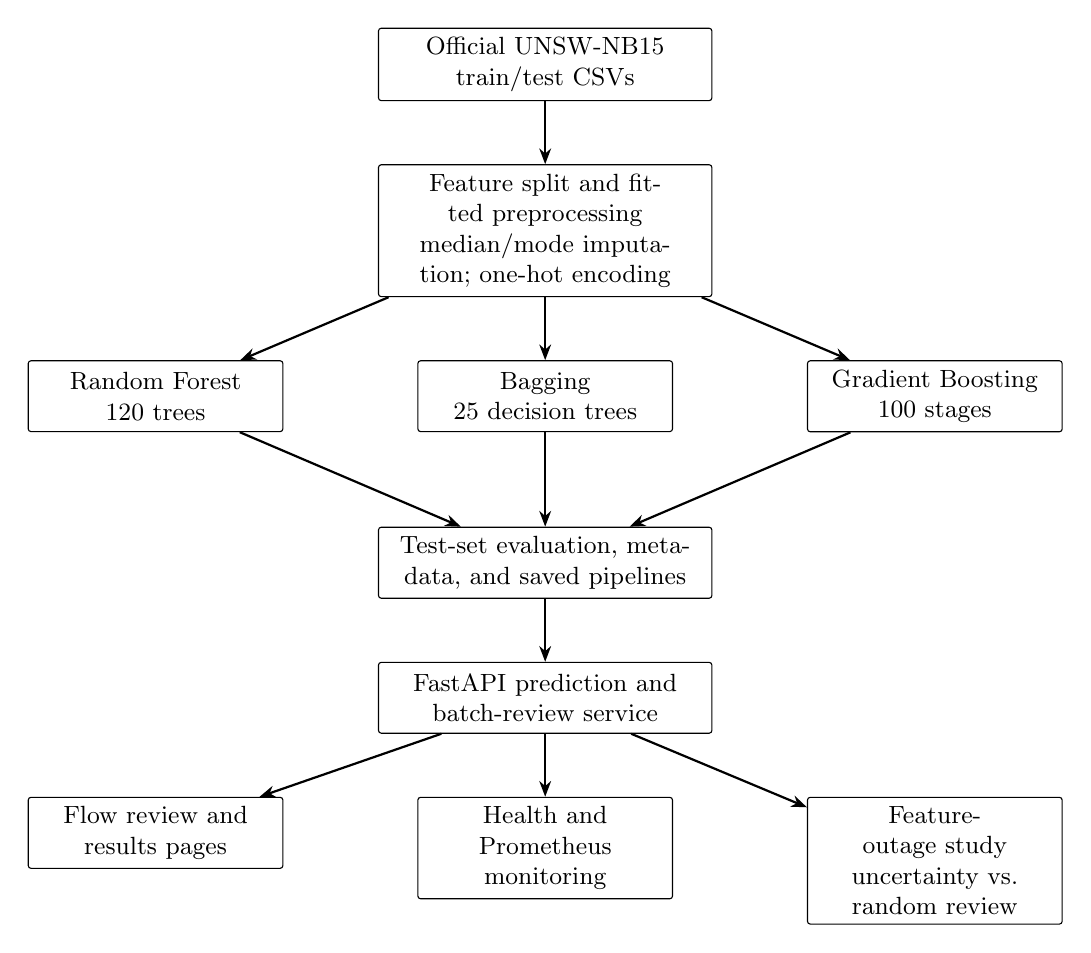
\begin{tikzpicture}[
  node distance=8mm and 12mm,
  block/.style={draw, rounded corners=1pt, align=center, minimum height=9mm, text width=30mm, font=\small},
  wide/.style={draw, rounded corners=1pt, align=center, minimum height=9mm, text width=40mm, font=\small},
  arrow/.style={-{Stealth[length=2mm]}, thick}
]
\node[wide] (data) {Official UNSW-NB15 train/test CSVs};
\node[wide, below=of data] (prep) {Feature split and fitted preprocessing\\median/mode imputation; one-hot encoding};
\node[block, below left=of prep] (rf) {Random Forest\\120 trees};
\node[block, below=of prep] (bag) {Bagging\\25 decision trees};
\node[block, below right=of prep] (gb) {Gradient Boosting\\100 stages};
\node[wide, below=12mm of bag] (reports) {Test-set evaluation, metadata, and saved pipelines};
\node[wide, below=of reports] (api) {FastAPI prediction and batch-review service};
\node[block, below left=of api] (web) {Flow review and results pages};
\node[block, below=of api] (mon) {Health and Prometheus monitoring};
\node[block, below right=of api] (study) {Feature-outage study\\uncertainty vs. random review};
\draw[arrow] (data) -- (prep);
\draw[arrow] (prep) -- (rf);
\draw[arrow] (prep) -- (bag);
\draw[arrow] (prep) -- (gb);
\draw[arrow] (rf) -- (reports);
\draw[arrow] (bag) -- (reports);
\draw[arrow] (gb) -- (reports);
\draw[arrow] (reports) -- (api);
\draw[arrow] (api) -- (web);
\draw[arrow] (api) -- (mon);
\draw[arrow] (api) -- (study);
\end{tikzpicture}
\caption{CyberSentinel-ML separates model fitting and ordinary held-out evaluation from a repeated feature-outage review experiment. The API serves trained pipelines; the research path evaluates review selection on labeled test records.}
\label{fig:architecture}
\end{figure*}

\section{Experimental Method}
\subsection{Classifier Evaluation}
The primary model comparison uses the official train/test split without altering its rows. Each fitted pipeline returns an attack score $s_i$ for test flow $i$. The binary decision is
\begin{equation}
\hat{y}_i = \mathbb{1}[s_i \geq 0.55].
\end{equation}
Accuracy, attack precision, attack recall, attack F1, and ROC-AUC are reported. Threshold-dependent metrics and confusion matrices use the common threshold of 0.55; ROC-AUC is computed from continuous scores and is threshold independent. The threshold was fixed for this report, not selected from the test set.

For the attack class, precision is $TP/(TP+FP)$ and recall is $TP/(TP+FN)$. The F1-score is their harmonic mean, $2PR/(P+R)$. The false-positive rate is $FP/(FP+TN)$, and the false-negative rate is $FN/(FN+TP)$. These rates describe different operational costs: false positives add benign flows to an alert queue, whereas false negatives are attacks left without an attack label. ROC-AUC summarizes score ranking over possible thresholds; it does not specify the error counts at 0.55. The model probabilities have not undergone a separate calibration procedure, so scores are used for ranking and thresholding rather than interpreted as calibrated real-world risks.

The model comparison fits one model of each type at random seed 42. It is a point-estimate benchmark comparison, not a repeated model-selection experiment. The five-seed protocol belongs to the separate triage study and should not be conflated with the classifier table.

\subsection{Feature-Group Outages}
The review experiment fits a fresh Random Forest for each of five seeds (42--46) using the clean training partition. Ten test conditions are evaluated: the clean condition and nine feature-group outages. In each outage condition, all selected columns are replaced by missing values in the test rows, while the training data remain unchanged. The preprocessing pipeline imputes the missing values using statistics learned from clean training data. The groups are protocol context; packet counts; byte volume; timing; TTL/state; TCP; connection counts; application fields; and packet loss. The experiment therefore represents an inference-time availability shift, not retraining on a reduced feature set.

Table~\ref{tab:outage_groups} records the columns hidden in each simulated outage. The groups are defined to correspond to broad traffic-measurement families rather than individual features. That design asks whether removing a related block of evidence changes the usefulness of the review queue. It also means that an outage can remove fields with different scales and predictive roles; the experiment does not isolate the causal contribution of any single field.

\begin{table*}[t]
\caption{Feature groups used in the inference-time outage simulation.}
\label{tab:outage_groups}
\centering
\small
\begin{tabular}{lp{0.76\textwidth}}
\toprule
Group & Fields replaced with missing values \\
\midrule
Protocol context & \texttt{proto}, \texttt{service}, \texttt{state} \\
Packet counts & \texttt{spkts}, \texttt{dpkts} \\
Byte volume & \texttt{sbytes}, \texttt{dbytes}, \texttt{sload}, \texttt{dload}, \texttt{smean}, \texttt{dmean} \\
Timing & \texttt{dur}, \texttt{rate}, \texttt{sinpkt}, \texttt{dinpkt}, \texttt{sjit}, \texttt{djit} \\
TTL/state & \texttt{sttl}, \texttt{dttl}, \texttt{ct\_state\_ttl} \\
TCP & \texttt{swin}, \texttt{stcpb}, \texttt{dtcpb}, \texttt{dwin}, \texttt{tcprtt}, \texttt{synack}, \texttt{ackdat} \\
Connection counts & \texttt{ct\_srv\_src}, \texttt{ct\_dst\_ltm}, \texttt{ct\_src\_dport\_ltm}, \texttt{ct\_dst\_sport\_ltm}, \texttt{ct\_dst\_src\_ltm}, \texttt{ct\_src\_ltm}, \texttt{ct\_srv\_dst} \\
Application & \texttt{trans\_depth}, \texttt{response\_body\_len}, \texttt{is\_ftp\_login}, \texttt{ct\_ftp\_cmd}, \texttt{ct\_flw\_http\_mthd}, \texttt{is\_sm\_ips\_ports} \\
Packet loss & \texttt{sloss}, \texttt{dloss} \\
\bottomrule
\end{tabular}
\end{table*}

\begin{figure*}[t]
\centering
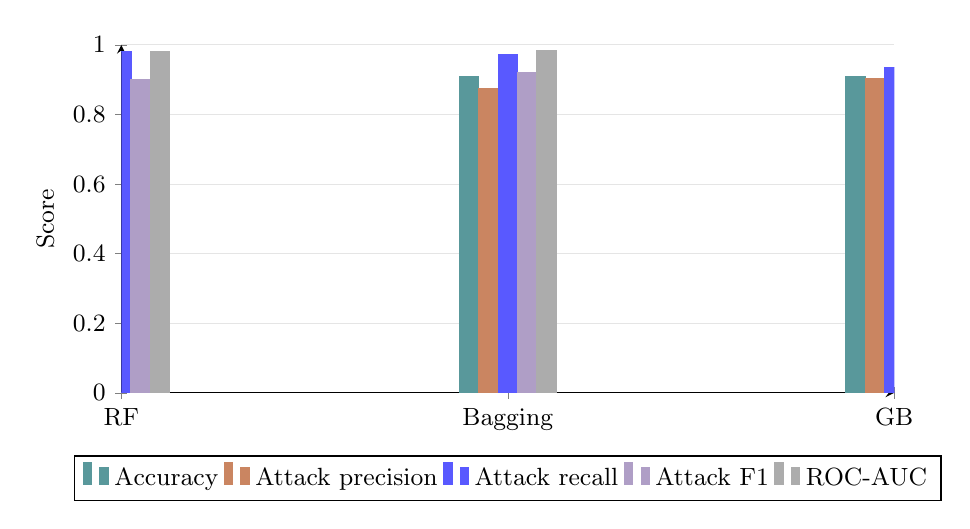
\begin{tikzpicture}
\begin{axis}[
  ybar,
  bar width=7pt,
  width=0.94\textwidth,
  height=6cm,
  ymin=0, ymax=1,
  ylabel={Score},
  symbolic x coords={RF,Bagging,GB},
  xtick=data,
  enlarge x limits=0.22,
  axis lines=left,
  ymajorgrids=true,
  grid style={gray!20},
  legend style={at={(0.5,-0.18)},anchor=north,legend columns=5,font=\small},
  tick label style={font=\small},
  label style={font=\small},
]
\addplot+[fill=modelteal!70,draw=modelteal!70,bar shift=-14pt] coordinates {(RF,0.8815) (Bagging,0.9080) (GB,0.9092)};
\addlegendentry{Accuracy}
\addplot+[fill=modelorange!75,draw=modelorange!75,bar shift=-7pt] coordinates {(RF,0.8328) (Bagging,0.8751) (GB,0.9043)};
\addlegendentry{Attack precision}
\addplot+[fill=blue!65,draw=blue!65,bar shift=0pt] coordinates {(RF,0.9819) (Bagging,0.9716) (GB,0.9339)};
\addlegendentry{Attack recall}
\addplot+[fill=modelviolet!60,draw=modelviolet!60,bar shift=7pt] coordinates {(RF,0.9012) (Bagging,0.9209) (GB,0.9189)};
\addlegendentry{Attack F1}
\addplot+[fill=gray!65,draw=gray!65,bar shift=14pt] coordinates {(RF,0.9798) (Bagging,0.9825) (GB,0.9775)};
\addlegendentry{ROC-AUC}
\end{axis}
\end{tikzpicture}
\caption{Threshold-dependent classification scores and threshold-independent ROC-AUC. The vertical axis begins at zero.}
\label{fig:model_metrics}
\end{figure*}

The visual comparison in Fig.~\ref{fig:model_metrics} reinforces that all three models rank test examples well by ROC-AUC, while their threshold-specific behavior differs. The small visual separation in accuracy should not distract from the larger differences in error type. A decision-maker who prioritizes detection may accept more false alarms; a queue with a hard analyst capacity may prefer higher precision or a lower false-positive rate.

For each condition, the model predicts all 82,332 test rows at threshold 0.55. The review policy selects
\begin{equation}
R = \left\lfloor 0.10N \right\rfloor = 8{,}233
\end{equation}
rows with the smallest absolute score margin $|s_i-0.55|$. A reviewed error is a row for which the binary prediction differs from the test label. For the random baseline, 200 uniform samples without replacement of size $R$ are drawn per seed and condition. The test labels do not affect which records either policy selects.

The primary comparison is the paired difference in the number of errors captured by uncertainty review and the mean number captured by random review, computed for each seed. The report gives the mean paired lift and an exact two-sided sign test across the five seed-level differences. Benjamini--Hochberg adjustment is then applied across the scenario and category sign-test comparisons. Attack-category summaries use \texttt{attack\_cat} after queue selection; they are descriptive subgroup analyses, not separate model inputs. A small category error count can make a capture percentage unstable or undefined.

\section{Results}
\subsection{Model Comparison}
Table~\ref{tab:model_metrics} shows the saved test-set results. Gradient Boosting achieved the highest accuracy and attack precision, Bagging achieved the highest attack F1 and ROC-AUC, and Random Forest achieved the highest attack recall. This is a practical trade-off: the Random Forest found 44,510 of 45,332 attacks but also generated 8,934 false alarms. Gradient Boosting produced fewer false alarms (4,479) at the cost of more missed attacks (2,995). No single metric makes one model preferable for every deployment objective.

\begin{table*}[t]
\caption{Classifier results on the official UNSW-NB15 test split at threshold 0.55.}
\label{tab:model_metrics}
\centering
\small
\begin{tabular}{lrrrrrr}
\toprule
Model & Accuracy & Attack precision & Attack recall & Attack F1 & ROC-AUC & Threshold \\
\midrule
Random Forest & 0.8815 & 0.8328 & \textbf{0.9819} & 0.9012 & 0.9798 & 0.55 \\
Bagging & 0.9080 & 0.8751 & 0.9716 & \textbf{0.9209} & \textbf{0.9825} & 0.55 \\
Gradient Boosting & \textbf{0.9092} & \textbf{0.9043} & 0.9339 & 0.9189 & 0.9775 & 0.55 \\
\bottomrule
\end{tabular}
\end{table*}

\begin{table*}[t]
\caption{Confusion matrices for the three classifiers at threshold 0.55.}
\label{tab:confusions}
\centering
\small
\begin{tabular}{lrrrr}
\toprule
Model & True negative & False positive & False negative & True positive \\
\midrule
Random Forest & 28,066 & 8,934 & 822 & 44,510 \\
Bagging & 30,715 & 6,285 & 1,286 & 44,046 \\
Gradient Boosting & 32,521 & 4,479 & 2,995 & 42,337 \\
\bottomrule
\end{tabular}
\end{table*}

The confusion matrices can also be read as rates. Random Forest's false-positive rate is 24.15\% and its false-negative rate is 1.81\%. Bagging reduces the false-positive rate to 16.99\%, with a 2.84\% false-negative rate. Gradient Boosting has the lowest false-positive rate (12.11\%) and highest false-negative rate (6.61\%) among these models. This exchange is consistent with the precision/recall pattern and makes threshold selection a policy decision rather than a search for a universally best score.

\begin{figure}[t]
\centering
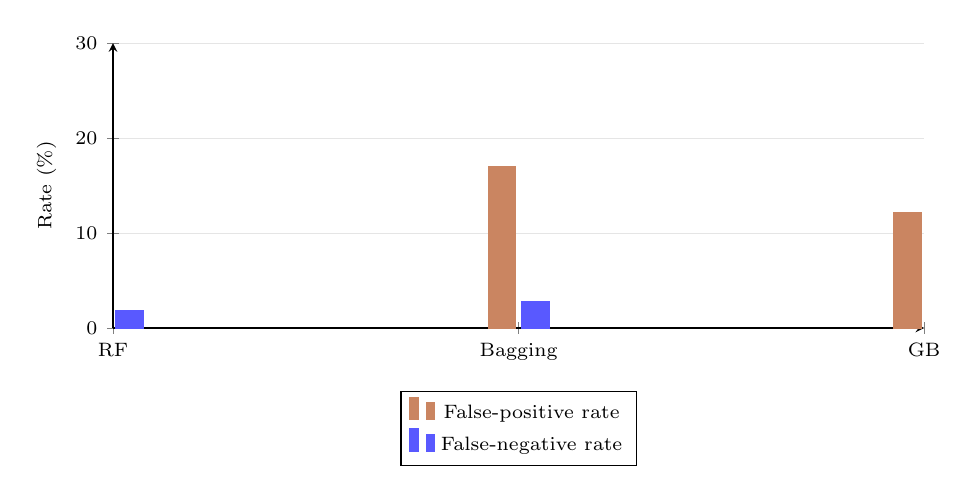
\begin{tikzpicture}
\begin{axis}[
  ybar,
  bar width=10pt,
  width=0.98\columnwidth,
  height=5.2cm,
  ymin=0, ymax=30,
  ylabel={Rate (\%)},
  symbolic x coords={RF,Bagging,GB},
  xtick=data,
  enlarge x limits=0.25,
  axis lines=left,
  ymajorgrids=true,
  grid style={gray!20},
  legend style={at={(0.5,-0.22)},anchor=north,legend columns=1,font=\scriptsize},
  tick label style={font=\scriptsize},
  label style={font=\scriptsize},
]
\addplot+[fill=modelorange!75,draw=modelorange!75,bar shift=-6pt] coordinates {(RF,24.15) (Bagging,16.99) (GB,12.11)};
\addlegendentry{False-positive rate}
\addplot+[fill=blue!65,draw=blue!65,bar shift=6pt] coordinates {(RF,1.81) (Bagging,2.84) (GB,6.61)};
\addlegendentry{False-negative rate}
\end{axis}
\end{tikzpicture}
\caption{False-positive and false-negative rates at threshold 0.55.}
\label{fig:error_rates}
\end{figure}

\subsection{Review under Feature Outages}
The ten conditions produced mean uncertainty-review lifts over the random baseline ranging from approximately 2,791 to 4,331 errors per reviewed batch. Table~\ref{tab:outage_results} reports all scenarios, and Fig.~\ref{fig:outage_lift} compares their mean lifts. The clean condition is also summarized in Table~\ref{tab:triage}. The uncertainty queue captured about 39.9\% of all clean-condition errors while reviewing 10\% of the test rows. The random queue captured about 10.0\% of errors on average, as expected for a uniform sample. All five seeds had positive lift in the clean condition, and this direction was consistent in all feature-outage conditions.

\begin{table*}[t]
\caption{Mean test-set results by feature-availability condition, aggregated over five training seeds.}
\label{tab:outage_results}
\centering
\scriptsize
\begin{tabular}{lrrrrrr}
\toprule
Condition & Baseline accuracy & Baseline errors & Uncertainty caught & Random mean caught & Lift & Adjusted $q$ \\
\midrule
Clean & 0.8815 & 9,759.0 & 3,891.8 & 976.0 & 2,915.8 & 0.0948 \\
Protocol context & 0.8606 & 11,478.8 & 4,410.6 & 1,147.2 & 3,263.4 & 0.0948 \\
Packet counts & 0.8706 & 10,653.6 & 4,058.2 & 1,064.3 & 2,993.9 & 0.0948 \\
Byte volume & 0.8202 & 14,807.0 & 5,811.2 & 1,480.4 & 4,330.8 & 0.0948 \\
Timing & 0.8319 & 13,841.4 & 5,279.6 & 1,382.2 & 3,897.4 & 0.0948 \\
TTL/state & 0.8402 & 13,157.6 & 4,107.6 & 1,316.6 & 2,791.0 & 0.0948 \\
TCP & 0.8194 & 14,870.0 & 5,003.2 & 1,485.1 & 3,518.1 & 0.0948 \\
Connection counts & 0.8793 & 9,934.2 & 3,853.0 & 994.2 & 2,858.8 & 0.0948 \\
Application & 0.8838 & 9,567.4 & 3,871.4 & 957.4 & 2,914.0 & 0.0948 \\
Packet loss & 0.8658 & 11,048.2 & 4,234.6 & 1,105.1 & 3,129.5 & 0.0948 \\
\bottomrule
\end{tabular}
\end{table*}

\begin{figure*}[t]
\centering
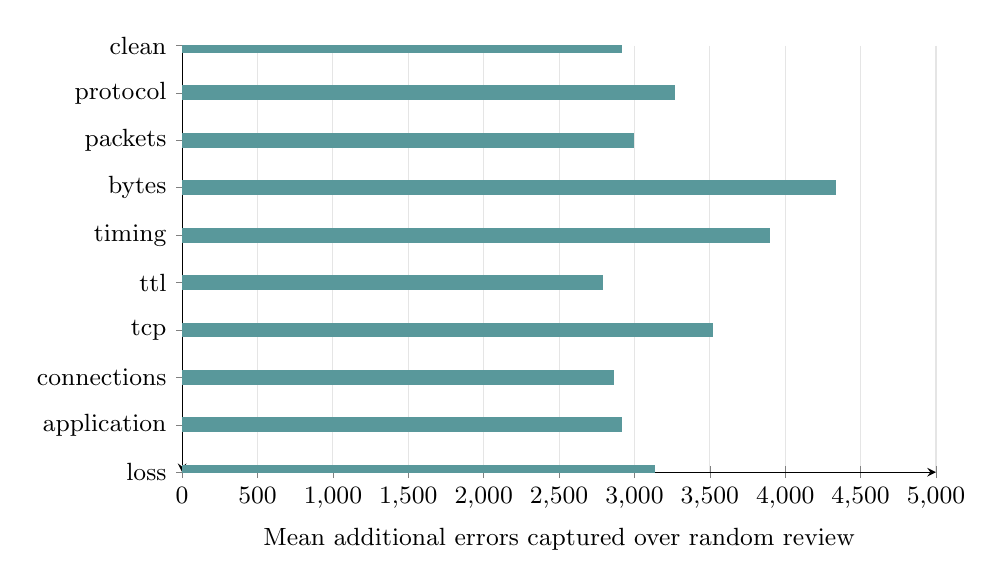
\begin{tikzpicture}
\begin{axis}[
  xbar,
  width=0.92\textwidth,
  height=7cm,
  xmin=0, xmax=5000,
  xlabel={Mean additional errors captured over random review},
  symbolic y coords={clean,protocol,packets,bytes,timing,ttl,tcp,connections,application,loss},
  ytick=data,
  y dir=reverse,
  axis lines=left,
  xmajorgrids=true,
  grid style={gray!20},
  bar width=5pt,
  tick label style={font=\small},
  label style={font=\small},
]
\addplot+[fill=modelteal!70,draw=modelteal!70] coordinates {
  (2915.8,clean) (3263.4,protocol) (2993.9,packets) (4330.8,bytes)
  (3897.4,timing) (2791.0,ttl) (3518.1,tcp) (2858.8,connections)
  (2914.0,application) (3129.5,loss)
};
\end{axis}
\end{tikzpicture}
\caption{Mean lift in errors captured by uncertainty review compared with 200 equal-size random draws. Each bar averages five model seeds; the feature outage is applied to the test rows only.}
\label{fig:outage_lift}
\end{figure*}

Byte-volume outage yielded the largest mean absolute lift (4,330.8 errors), while TTL/state outage yielded the smallest (2,791.0). This ordering should not be interpreted as a direct ranking of feature-group importance. The number of errors available to capture changes across conditions: byte-volume and TCP outages increased the baseline error count to roughly 14,800, whereas application outage produced 9,567.4 errors, slightly fewer than the clean condition. The lift therefore reflects both how many errors exist and how effectively the review ranking concentrates them. The lower application-outage error count also cautions against assuming that every missing field group must degrade every model metric; correlated predictors and the learned tree structure can produce non-monotonic effects.

\begin{table}[t]
\caption{Clean-feature review result; counts are means across five seeds except for test-set size.}
\label{tab:triage}
\centering
\small
\begin{tabular}{lr}
\toprule
Quantity & Value \\
\midrule
Test rows & 82,332 \\
Rows reviewed (10\%) & 8,233 \\
Baseline model errors & 9,759.0 \\
Errors in uncertainty queue & 3,891.8 \\
Errors in random queue (mean of 200 draws) & 976.0 \\
Mean lift over random review & 2,915.8 \\
Seeds with positive lift & 5/5 \\
Exact sign-test $p$-value & 0.0625 \\
Adjusted $q$-value & 0.0948 \\
\bottomrule
\end{tabular}
\end{table}

For the clean condition, none of the 200 random draws captured as many errors as uncertainty review. With the experiment's add-one correction, the conditional randomization tail estimate is $(0+1)/(200+1)=0.00498$. This answers a narrower question: given these fitted scores and this test set, how often did a same-size random queue do at least as well? It does not replace the seed-level analysis, because the random draws reuse the same model predictions and labeled records. The paired exact sign test across five fitted seeds gives $p=0.0625$, and the adjusted scenario value is $q=0.0948$. The result should therefore not be called statistically significant at the conventional 0.05 level after the reported correction. The 200-draw randomization estimate also has limited resolution, and five fits are a small basis for generalization claims.

\subsection{Attack-Category Variation}
Category-level counts show why the aggregate review lift should not be read as uniform across attacks. Table~\ref{tab:categories} reports selected clean-condition categories. Uncertainty review captured a large share of Fuzzers and Exploits errors in this split, while other categories had very few baseline errors. Normal traffic is included because false positives are model errors and consume review capacity. The apparent 100\% capture for Analysis in some seed averages corresponds to fewer than one mean error and is not strong evidence of a reliable category effect. Across scenario and category comparisons, adjusted values did not cross 0.05.

\begin{table*}[t]
\caption{Selected clean-condition category results; error counts are averages across five seeds.}
\label{tab:categories}
\centering
\small
\begin{tabular}{lrrrrr}
\toprule
Category & Rows & Baseline errors & Uncertainty errors caught & Random mean caught & Adjusted $q$ \\
\midrule
Normal & 37,000 & 8,936.4 & 3,354.8 & 894.2 & 0.0948 \\
Fuzzers & 6,062 & 753.6 & 493.6 & 75.0 & 0.0948 \\
Exploits & 11,132 & 56.8 & 34.2 & 5.6 & 0.0948 \\
DoS & 4,089 & 5.0 & 3.6 & 0.5 & 0.0948 \\
Analysis & 677 & 0.6 & 0.6 & 0.1 & 0.5802 \\
Backdoor & 583 & 0.0 & 0.0 & 0.0 & n/a \\
\bottomrule
\end{tabular}
\end{table*}

\begin{figure*}[t]
\centering
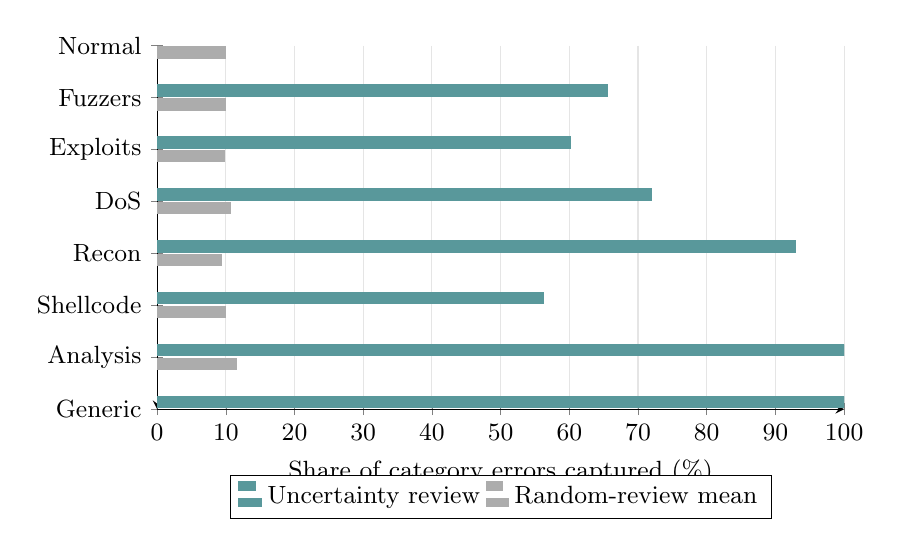
\begin{tikzpicture}
\begin{axis}[
  xbar,
  width=0.85\textwidth,
  height=6.2cm,
  xmin=0, xmax=100,
  xlabel={Share of category errors captured (\%)},
  symbolic y coords={Normal,Fuzzers,Exploits,DoS,Recon,Shellcode,Analysis,Generic},
  ytick=data,
  y dir=reverse,
  enlarge y limits=0.08,
  axis lines=left,
  xmajorgrids=true,
  grid style={gray!20},
  bar width=4pt,
  legend style={at={(0.5,-0.18)},anchor=north,legend columns=2,font=\small},
  tick label style={font=\small},
  label style={font=\small},
]
\addplot+[fill=modelteal!70,draw=modelteal!70,bar shift=2.5pt] coordinates {
  (37.5,Normal) (65.5,Fuzzers) (60.2,Exploits) (72.0,DoS)
  (92.9,Recon) (56.2,Shellcode) (100.0,Analysis) (100.0,Generic)
};
\addlegendentry{Uncertainty review}
\addplot+[fill=gray!65,draw=gray!65,bar shift=-2.5pt] coordinates {
  (10.0,Normal) (10.0,Fuzzers) (9.8,Exploits) (10.6,DoS)
  (9.3,Recon) (10.0,Shellcode) (11.5,Analysis) (10.0,Generic)
};
\addlegendentry{Random-review mean}
\end{axis}
\end{tikzpicture}
\caption{Within-category error capture rates in the clean condition. The 10\% budget applies to the complete test batch, not separately to each category. Analysis, Generic, DoS, Reconnaissance, and Shellcode have very small baseline error counts in this run; their rates are unstable.}
\label{fig:category_capture}
\end{figure*}

The larger categories account for most of the overall lift. In particular, the aggregate capture advantage is driven by Normal and Fuzzers errors in absolute count, with a smaller but clear count difference for Exploits. Fig.~\ref{fig:category_capture} makes the within-category rates easier to compare, but the apparently high rates for Analysis and Generic each reflect less than one mean error across seeds. These estimates are intrinsically unstable and should not be read as reliable evidence of category-specific performance. The category table and graph expose variation for follow-up study; they do not rank attack families by detector quality.

\subsection{Feature-Importance Context}
The saved Random Forest grouped-importance report provides a descriptive view of what the fitted model used. The highest-ranked groups were \texttt{sttl} (8.34\%), \texttt{ct\_state\_ttl} (5.80\%), \texttt{sload} (5.28\%), \texttt{rate} (5.20\%), and \texttt{dload} (5.05\%). Together, the ten highest-ranked groups account for about 47.3\% of the reported impurity importance. This overlaps with several outage families, but importance and outage sensitivity are different quantities: feature importance describes split usage in one fitted forest, while outage evaluation measures the full model's resulting test errors after an entire group is hidden.

\begin{figure}[t]
\centering
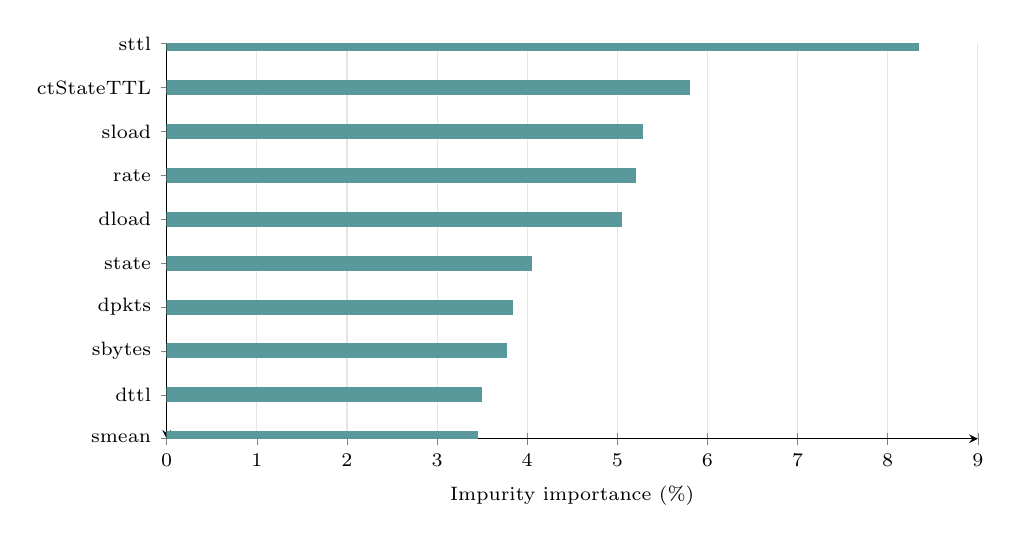
\begin{tikzpicture}
\begin{axis}[
  xbar,
  width=0.98\columnwidth,
  height=6.6cm,
  xmin=0, xmax=9,
  xlabel={Impurity importance (\%)},
  symbolic y coords={sttl,ctStateTTL,sload,rate,dload,state,dpkts,sbytes,dttl,smean},
  ytick=data,
  y dir=reverse,
  axis lines=left,
  xmajorgrids=true,
  grid style={gray!20},
  bar width=5pt,
  tick label style={font=\scriptsize},
  label style={font=\scriptsize},
]
\addplot+[fill=modelteal!70,draw=modelteal!70] coordinates {
  (8.34,sttl) (5.80,ctStateTTL) (5.28,sload) (5.20,rate) (5.05,dload)
  (4.05,state) (3.84,dpkts) (3.77,sbytes) (3.49,dttl) (3.45,smean)
};
\end{axis}
\end{tikzpicture}
\caption{Ten highest grouped impurity-importance values for the Random Forest. The label \texttt{ctStateTTL} abbreviates \texttt{ct\_state\_ttl}.}
\label{fig:importance}
\end{figure}

Impurity-based importance is not a causal explanation and can favor features with particular split opportunities or correlated alternatives. The ranking should therefore be used to guide inspection, not as evidence that a field causes an attack or that removing the highest-ranked field alone would reproduce a grouped outage result. The full ranking and analysis are available in the repository's CSV and Markdown reports.

\section{Discussion}
The classifier comparison illustrates the cost of optimizing one metric in isolation. Random Forest is a reasonable default when missing attacks are especially costly, given its 0.9819 recall at this threshold. That comes with the largest false-positive count among the three evaluated models. Gradient Boosting has the highest precision and the fewest false alarms, but its recall is lower. Bagging has the highest F1 and ROC-AUC in this run. A deployed system would need to set its threshold against a defined alert capacity and the relative cost of false positives and false negatives, then validate that operating point on data representative of its environment.

The review experiment suggests that score margins carry useful information about where this Random Forest makes errors. Under clean inputs, the fixed-budget uncertainty queue found about four times as many errors as a random queue of equal size. Similar positive mean lifts appeared under each simulated feature outage. This observation is relevant to human-in-the-loop triage: when model confidence is weak, a limited review budget may be better spent on those rows than on a uniform sample. However, the experiment does not demonstrate reduced incident response time, analyst productivity, or improved security outcomes. No human reviewers participated, and the test set is a benchmark rather than operational traffic.

The category breakdown also argues against a single global interpretation. The uncertainty policy's allocation among categories is a consequence of the model's scores and category prevalence. A category with few errors may show a high capture fraction by chance; a category with many records may contribute many captured errors while receiving a small within-category review fraction. Future studies should report both counts and rates, retain per-seed measurements, and obtain additional independent data before making category-specific claims.

\section{Limitations and Threats to Validity}
Several limits define the scope of these results. First, all findings come from one benchmark dataset and its supplied split. They do not establish performance on contemporary enterprise traffic, a different collection period, or a different network. Second, the outage study simulates missingness by replacing whole feature groups with null values at test time. Real telemetry failures can be selective, correlated with device or attack type, or accompanied by schema changes; those conditions are not represented here.

Third, the study trains on clean inputs and tests under outages. This is intentional because the question concerns unexpected feature loss, but it should not be confused with a model trained to tolerate missing groups. Fourth, classifier hyperparameters are fixed project defaults rather than the result of nested validation or a broad search. Fifth, the review threshold and workload are fixed at 0.55 and 10\%, respectively. Other operating points may change both the amount of baseline error and the advantage of uncertainty review.

Finally, the primary inferential analysis uses only five training seeds. An exact two-sided sign test with five nonzero observations cannot return a $p$-value below 0.0625 even if every seed favors one policy. The Benjamini--Hochberg correction further raises the criterion for declaring a result. The current adjusted $q$-values therefore indicate that the observed pattern warrants additional evaluation, not that the experiment has established a statistically significant effect. Category subgroups are especially limited by small numbers of errors and shared test rows across scenarios.

\section{Reproducibility and Availability}
The code, report inputs, and commands are maintained in the CyberSentinel-ML repository. The raw dataset and trained model binaries are not included; users must obtain the UNSW-NB15 files from the dataset authors and retrain locally. With Python 3.12 and the repository's requirements installed, the primary commands are:

\begin{verbatim}
python -m src.train --model all --threshold 0.55
python -m src.visualize_results
python -m src.robustness_experiment --review-budget 0.10 --decision-threshold 0.55
python -m uvicorn app.main:app --host 127.0.0.1 --port 8000
\end{verbatim}

The training report is written to \texttt{reports/training\_results.json} and Markdown; the review experiment writes JSON and CSV reports under \texttt{reports/}. The website exposes flow review at \texttt{/}, model comparisons at \texttt{/results}, and the feature-outage study at \texttt{/research/feature-outages}. The UNSW-NB15 data files must be placed under \texttt{data/Training and Testing Sets/} or selected using the \texttt{UNSW\_NB15\_DATA\_DIR} environment variable.

\section{Conclusion}
This paper presented a reproducible binary flow-classification system and a controlled review-budget experiment on the official UNSW-NB15 split. The model comparison exposed distinct operating trade-offs among Random Forest, Bagging, and Gradient Boosting. In the clean-feature condition, uncertainty-ranked review captured substantially more model errors than an equal-size random queue, and the mean lift remained positive across five seeds and simulated feature-group outages. The category breakdown showed that this benefit was concentrated in categories with enough errors to measure, while rare categories remained inconclusive.

The statistical evidence is not conclusive at a 0.05 threshold after correction. The next useful step is not to increase the strength of the claim, but to repeat the protocol on additional seeds and an independent dataset, model realistic telemetry failures, and assess whether analyst review of uncertainty-ranked records changes response quality. Until then, these results should be treated as a benchmark-specific finding and the system as a research prototype.

\begin{thebibliography}{00}
\bibitem{moustafa2015}
N. Moustafa and J. Slay, ``UNSW-NB15: A comprehensive data set for network intrusion detection systems (UNSW-NB15 network data set),'' in \emph{Proc. Military Communications and Information Systems Conference (MilCIS)}, 2015, pp. 1--6, doi: 10.1109/MILCIS.2015.7348942.

\bibitem{unswsite}
UNSW Canberra, ``The UNSW-NB15 dataset.'' [Online]. Available: \url{https://research.unsw.edu.au/projects/unsw-nb15-dataset}. Accessed: Nov. 1, 2026.

\bibitem{breiman2001}
L. Breiman, ``Random forests,'' \emph{Machine Learning}, vol. 45, no. 1, pp. 5--32, 2001, doi: 10.1023/A:1010933404324.

\bibitem{breiman1996}
L. Breiman, ``Bagging predictors,'' \emph{Machine Learning}, vol. 24, no. 2, pp. 123--140, 1996, doi: 10.1007/BF00058655.

\bibitem{friedman2001}
J. H. Friedman, ``Greedy function approximation: A gradient boosting machine,'' \emph{The Annals of Statistics}, vol. 29, no. 5, pp. 1189--1232, 2001, doi: 10.1214/aos/1013203451.
\end{thebibliography}

\end{document}
